
\documentclass[11pt]{article}
\usepackage{geometry} % see geometry.pdf on how to lay out the page. There's lots.
\usepackage{amsmath}
\usepackage{amssymb}
\usepackage{hyperref}
\usepackage{easybmat}
\usepackage{epstopdf}
\usepackage{wrapfig}
\usepackage{graphicx}
\DeclareGraphicsRule{.tif}{png}{.png}{`convert #1 `dirname #1`/`basename #1 .tif`.png}

\geometry{a4paper} % or letter or a5paper or ... etc
% \geometry{landscape} % rotated page geometry

% See the ``Article customise'' template for come common customisations

\title{The Discrete Fourier Transform}
\author{Didi Park}
\date{13 May 2014}
%%% BEGIN DOCUMENT
\begin{document}

\maketitle

%%%%
\section{The Fourier Transform}
Let us define the Fourier transform $\hat{f}$, $f: \mathbb{R}\rightarrow\mathbb{C}$ to be
$$\hat{f}(\xi)=\int_{-\infty}^{\infty}f(x)e^{-2\pi i x \xi}\, \mathrm{d}x, \textrm{ for real }\xi.$$
$f(x)$ must be square integrable, that is,
$$\int_{-\infty}^{\infty} {\| f(x) \|}^2\,  \mathrm{d}x <\infty.$$

The Fourier transform also has an easy inverse:
$$f(x)=\int_{-\infty}^{\infty} \hat{f}(\xi)e^{2\pi i \xi x}\, \mathrm{d}\xi.$$

Speaking in linear algebra terms, the Fourier transform is a \emph{linear transformation}. This can easily be seen from the linearity and scalar multiplicity of the integral. Both the domain and codomain, $f$ and $\hat{f}$, effectively form infinite-dimensional vector spaces.
\subsection{Applications}
The Fourier transform relates a function's time or spatial domain to a frequency domain. 
It can be used to solve a wide variety of problems, including the following:
\begin{itemize}
\item Partial (and ordinary) differential equations: the Fourier transform of a function's derivative can be used to change a differential equation to an algebraic equation
\item Quantum mechanics: Fourier transforms on the solutions to Schr\"{o}dinger's equations form momentum space wave functions
\item Signal processing: Fourier transforms are employed to filter out noise
\item Data compression: JPEG's and mp3's, among other file formats, use Fourier transforms to compress data.
\end{itemize}

%%%%
\section{The Discrete Fourier Transform}
As you can see, the Fourier transform is continuous, making it difficult for computers to perform the transform to high accuracy. It also requires that the function being transformed be square integrable, thus limiting the possible inputs significantly.\\
The discrete fourier transform (DFT) is discrete, making it much more conducive to computation. Unlike the Fourier transform, it maps a countable set of numbers to a new countable set of numbers. If you're only interested in transforming a small set of data, use the DFT.
\subsection{Definition}
We simply discretize the Fourier transform by changing the integral to a sum, appropriately:
$$X_k=\sum_{n=0}^{N-1}x_n e^{-2\pi i n \frac{k}{N}}.$$
Note that the $\frac{k}{N}$ serves the same purpose as $\xi$ in the continuous case.\\
The inverse is given by:
$$ x_k = \frac{1}{N}\sum_{n=0}^{N-1}X_k e^{2\pi i n \frac{k}{N}}.$$
\subsection{Matrix representation}
The DFT, unsurprisingly, can be written as a matrix transformation.
$$
 F_n=\begin{pmatrix}
  1 && 1 && 1 && \dots && 1 \\
  1 && w && w^2 && \dots && w^{N-1}\\
  1 && w^2 && w^4 && \dots && w^{2(N-1)}\\
  \vdots && \vdots && \vdots && \dots &&\vdots \\
  1 && w^{N-1} && w^{2(N-1)} && \dots && w^{(N-1)^2} \\
 \end{pmatrix}$$
where $w=e^{i \frac{2\pi}{N}}$.\\
The inverse transform is given by:
$$ \frac{1}{N}F^*,$$ where * denotes the complex conjugate.\\
Notice that this matrix is symmetrical. In fact, its columns are also orthogonal (keep in mind that the complex dot product requires one to take the conjugate transpose).\\
These $w$'s can best be thought of as complex roots of unity.\\
\begin{figure}[h]
    \centering
    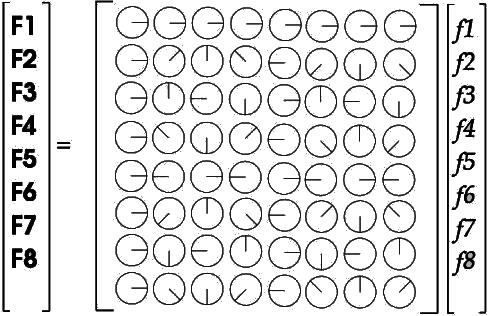
\includegraphics[scale=.45]{DFT_vis.jpg}
    \caption{The zeroth row transforms by the 0th roots, first row 1st roots, second row square roots, etc$.^{[6]}$}
\end{figure}

\section{The Fast Fourier Transform}
The DFT has efficiency $O(n^2)$. The fast Fourier transform (FFT) takes advantage of the symmetry and orthogonality of the DFT matrix, and recursively factors it until we reach an efficiency of $O(nlog(n)).$
Let us take the example of the $8\times8$ DFT matrix, $F_8$.
$$F_8=\begin{pmatrix}
  1 && D\\
  1 && -D\\
 \end{pmatrix}
 \begin{pmatrix}
  F_4 && 0\\
  0 && F_4\\
 \end{pmatrix}
 P_8
$$

Where
$$ \setcounter{MaxMatrixCols}{16}
   P_8=
   \begin{pmatrix}
   1 &&  0 && 0 && 0  && 0 && 0 && 0 && 0 \\
   0 && 0 && 0 && 0 && 1 && 0 && 0 && 0\\ 
   0 && 1 && 0 && 0 && 0 && 0 && 0 && 0\\
   0 && 0 && 0 && 0 && 0 && 1 && 0 && 0\\
   0 && 0 && 1 && 0 && 0 && 0 && 0 && 0\\
   0 && 0 && 0 && 0 && 0 && 0 && 1 && 0\\
   0 && 0 && 0 && 1 && 0 && 0 && 0 && 0\\
   0 && 0 && 0 && 0 && 0 && 0 && 0 && 1\\
 \end{pmatrix}, \, \,\,\,
 D=
  \begin{pmatrix}
   1 &&  0 && 0 && 0   \\
   0 && w && 0 && 0 \\ 
   0 && 1 && w^2 && 0\\
   0 && 0 && 0 && w^3 \\
 \end{pmatrix}.
 $$
 The permutation matrix splits the original $F_8$ into its even and odd columns. \\
Now we can recursively factorize by factorizing the $F_4$ matrices:
$$
\begin{pmatrix}
  1 && D\\
  1 && -D\\
 \end{pmatrix}
 \begin{pmatrix}
  \begin{matrix}1 && D\\ 1 && -D\\\end{matrix} && 0\\
  0 && \begin{matrix}1 && D\\ 1 && -D\\\end{matrix}\\
 \end{pmatrix} 
  \begin{pmatrix}
  \begin{matrix}F_{16} && 0\\ 0 && F_{16}\\\end{matrix} && 0\\
  0 && \begin{matrix}F_{16} && 0\\ 0 && F_{16}\\\end{matrix}\\
 \end{pmatrix} 
  \begin{pmatrix}
  P_4 && 0\\
  0 && P_4\\
 \end{pmatrix} 
 P_{64}
$$
\dots and 
we find that the efficiency of this process is $O(n log_2(n))$.
%%%%
\section{Further reading/Works Cited}
\begin{enumerate}
\item Strang, Gilbert. \emph{Lec 26, MIT 18.06 Linear Algebra.} \url{https://www.youtube.com/watch?v=M0Sa8fLOajA}
\item Tao, Terrence. \emph{An Epsilon of Room, I.} \url{https://terrytao.files.wordpress.com/2012/12/gsm-117-tao3-epsilon1.pdf.}
\item Terras, Audrey. (1999). \emph{Fourier Analysis on Finite Groups and Applications.}
\item Wikipedia. \emph{DFT Matrix}. \url{https://en.wikipedia.org/wiki/DFT_matrix}.
\item Wikipedia. \emph{Fourier Transform}. \url{https://en.wikipedia.org/wiki/Fourier_transform}
\item \url{http://math.berkeley.edu/~berlek/classes/CLASS.110/LECTURES/FFT}
item \emph{Digital Signal Processing/Discrete Fourier Transform. } \url{http://en.wikibooks.org/wiki/Digital_Signal_Processing/Discrete_Fourier_Transform}
\end{enumerate}
\vfill
  \centering
 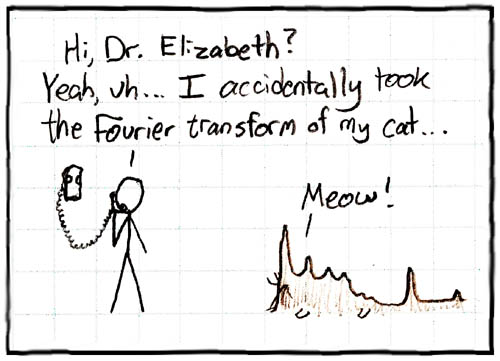
\includegraphics[scale=3]{fourier.jpg}\\
 \url{http://xkcd.com/26/}

\end{document}